%!TEX root = ./report.tex
\section{Solution}
\label{sec:solution}
The solution combines several open source technologies to attain an extensible solution with two reusable MWE2 client side workflows at its core. The setup allows the user to edit a subset of IFC in an auto-generated Eclipse editor in between the two workflows. The main model is stored on a BIMServer for merging, version control, and the possibility of collaboration through the client-server design pattern, as this section will explain further. The prototype serves as an open source alternative to similar, proprietary BIM software.

\subsection{IFC Meta Model}
% Our meta model is generated from ifcXML XSD, only handles ifcXML
% BIMServer - tightly coupled, but handles .ifc. Handles references as string
% Jim Steel model. Seems to be better, but we have no deserializer.
\label{subsec:ifc_meta_model}
The prototype uses a meta model for IFC that is auto-generated from the XML Schema Definition (XSD) of ifcXML.\footnote{ifcXML XSD: \url{http://buildingsmart-tech.org/ifcXML/IFC2x3/FINAL/IFC2X3.xsd}} This allows it to utilise the XML serialiser and deserialiser provided by EMF to convert ifcXML to and from its Java representation. The advantage of using these tools is that we are able to rely on well-tested and widely used software, thus removing the serialisation steps as potential sources of error. However, generating the meta model from an XSD also means that the client application of the prototype only supports ifcXML, and not  the more widely used IFC-EXPRESS format. Because BIMServer accepts and generates both formats, this is a minor concern. But it means that the client side of the prototype relies on BIMServer for IFC-EXPRESS handling.

Although we chose not to use it, BIMServer also provides a meta model for IFC. This meta model comes with a custom serialiser and deserialiser for IFC-EXPRESS. We found that using this model and the provided serialisation tools was undesirable, as it would mean that the client application of the prototype would be completely dependent on the BIMServer. An advantage of using this meta model would be that it resembles the documented IFC specification more closely than the auto-generated meta model (even though both are equally correct). Specifically, the BIMServer meta model models inverse relationships, which are not represented as intuitively in the auto-generated meta model.

A third meta model for IFC has been created by Jim Steel, Lecturer at the University of Queensland.\footnote{Jim Steel at the University of Queensland: \url{http://itee.uq.edu.au/~uqjstee8/}}\footnote{Jim Steel's model can be found at \url{http://www.emn.fr/z-info/atlanmod/index.php/Ecore#ifc2x3_0.1}} This meta model seems to model all relationships better than the two aforementioned models, but does not provide a deserialiser to any IFC format. As it is not within the scope of this project to create a deserialiser for such a meta model, it was not used. However, using this meta model could be considered as a future improvement.

\subsection{Pipes DSL}
\label{subsec:pipes_dsl}
Before moving into a more technical description of the workflows facilitating the final solution, we here present the simple Pipes DSL, which serves as the front-end of the prototype.

\begin{figure}[t]
    \centering
        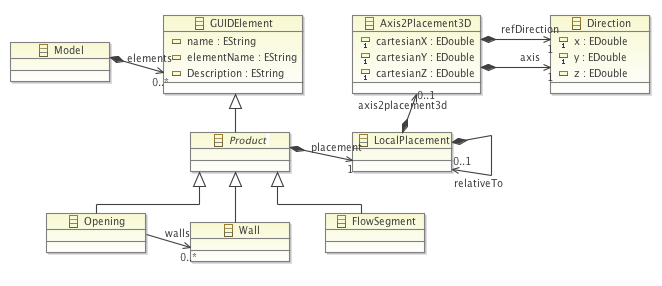
\includegraphics[width=110mm]{images/PipesEcoreModel.png}
    \caption{Pipes DSL Ecore meta model.}
    \label{fig:pipes_dsl_ecore_model}
\end{figure}

\begin{figure}[t]
    \centering
        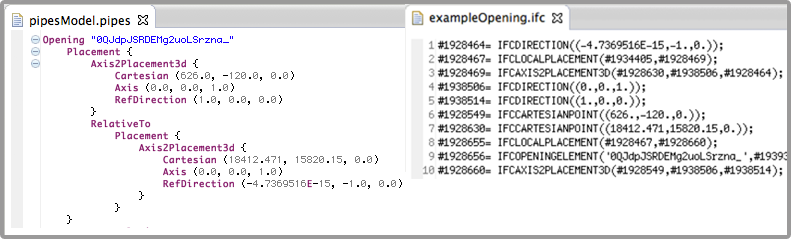
\includegraphics[width=120mm]{images/pipesAndExpressExample.png}
    \caption{A comparison of an opening specification in the Pipes DSL (left) and the IFC EXPRESS format (right) with placement references and metadata.}
    \label{fig:pipes_express_comparison}
\end{figure}

Figure \ref{fig:pipes_dsl_ecore_model} shows the Ecore model that the DSL is built upon. Compared to Figure \ref{fig:ifcheirachy}, all the critical elements of the domain are still present, but the inheritance hierarchy has been greatly simplified. As shown, Opening and Pipe are top level elements, each with a physical location specified by the LocalPlacement reference. Figure \ref{fig:pipes_express_comparison} depicts an example of an opening and a pipe as they are defined in the Pipes DSL in an uncluttered and manageable way, compared to the IFC-EXPRESS format. The textual syntax has been created from the Ecore meta model using Xtext, which also provides an editor with syntax highlighting and autocompletion.\footnote{For more information on Xtext, see \url{http://www.eclipse.org/Xtext/}} This editor is launched as an Eclipse instance.

\subsection{BIMServer}
The overall workflow of the end product is shown in Figure \ref{fig:overall_product_workflow}. As described in J\o rgensen's workflow document\,\cite{jorgensen12}, a construction model and a plumbing model are combined into one single model that needs to be verified. So-called openings, i.e. holes in walls and floors, need to be present where the plumbing model defines pipes to be installed. The merging of these models is executed on the BIMServer by the user as the first step of the workflow. When the models have been merged, the client application can retrieve the merged model as ifcXML. The user is now allowed to edit and add elements to the subset of the model on the client side before saving the building back to the BIMServer as ifcXML.

Note that the solution does not take concurrent editing by multiple clients into account, although BIMServer does support version control and change notifications for this exact purpose.

\begin{figure}[t]
    \centering
        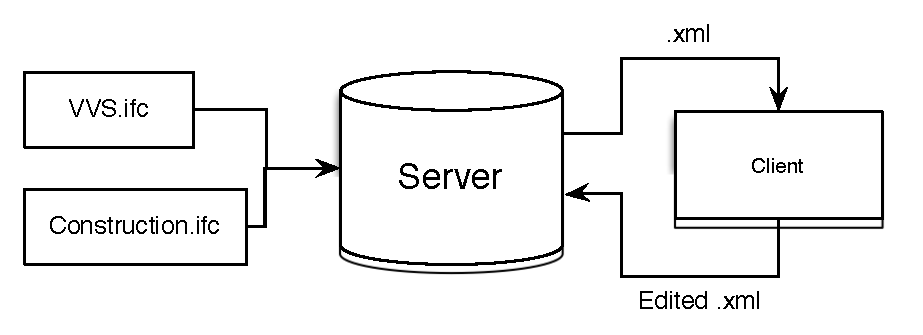
\includegraphics[width=70mm]{images/CompleteWorkflow.pdf}
    \caption{Overall product workflow starting with a merge of two models. The user can edit a subset of the model through the client-side application.}
    \label{fig:overall_product_workflow}
\end{figure}

Although many tools exist for this job, we let a BIMServer instance handle the initial merging of plumbing and construction models. An advantage of the BIMServer is that it also provides conversion tools, which allows the user to retrieve the saved building in other formats as well as a Java client library\,\cite{beetz10}.

\subsection{Client Side}
Figure \ref{fig:IFC2PipesWorkflow} shows the IFC to Pipes workflow retrieving an IFC model from the BIMServer as XML, processing it to the corresponding Java object graph, extracting the pipes and opening elements and converting these to an editable DSL instance, which is in turn saved to disk as an XMI file. The XML file loaded from the server is saved to the local disk for use by the second workflow explained below.

\begin{figure}[t]
    \centering
        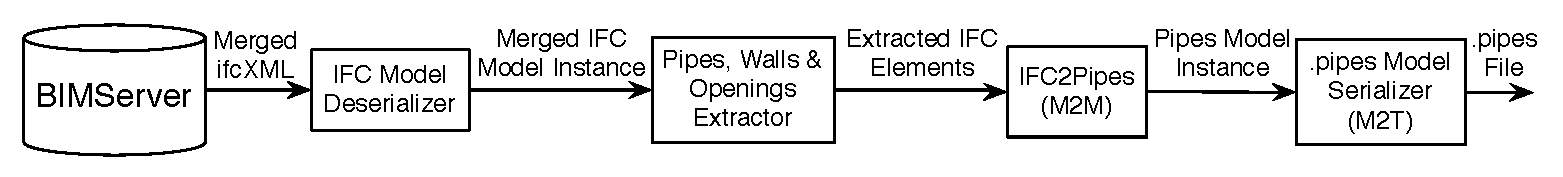
\includegraphics[width=114mm]{images/IFC2Pipes.pdf}
    \caption{Client-side workflow. Processes ifcXML from BIMServer and outputs a .pipes file, loadable in the Pipes DSL editor.}
    \label{fig:IFC2PipesWorkflow}
\end{figure}

The extraction process where relevant IFC elements are collected from the main model for conversion is implemented by a simple filtering mechanism extracting the pipe and opening elements. The real work of the IFC to Pipes workflow is done when this extract is converted to the corresponding Pipes DSL instance in the second to last step of the workflow. By utilizing the convenient model to model transformation language features of the Xtend language, each object is transformed from the IFC model to the corresponding PipesDSL object. Every IFC object inside the solution domain specified in Section \ref{subsec:problem_analysis} has a transformation rule specified here, making the conversion possible.

The second client side MWE2 workflow, Pipes to IFC, is depicted on Figure \ref{fig:Pipes2IFCWorkflow}, where the user-edited XMI file is loaded into a Main Model Updater workflow component together with the non-updated extracted instance of the main model. Notice how the extraction is loaded in using the same workflow modules as in the first workflow, except the XML file is not fetched from the server but from the local disk. This makes for an easier update process in the Main Model Updater as the extracted instance is guaranteed not to have changed while the user was editing the XMI file. After the main model instance has been updated to reflect the users changes it is converted to XML and this new file is saved back to the BIMServer.

\begin{figure}[t]
    \centering
        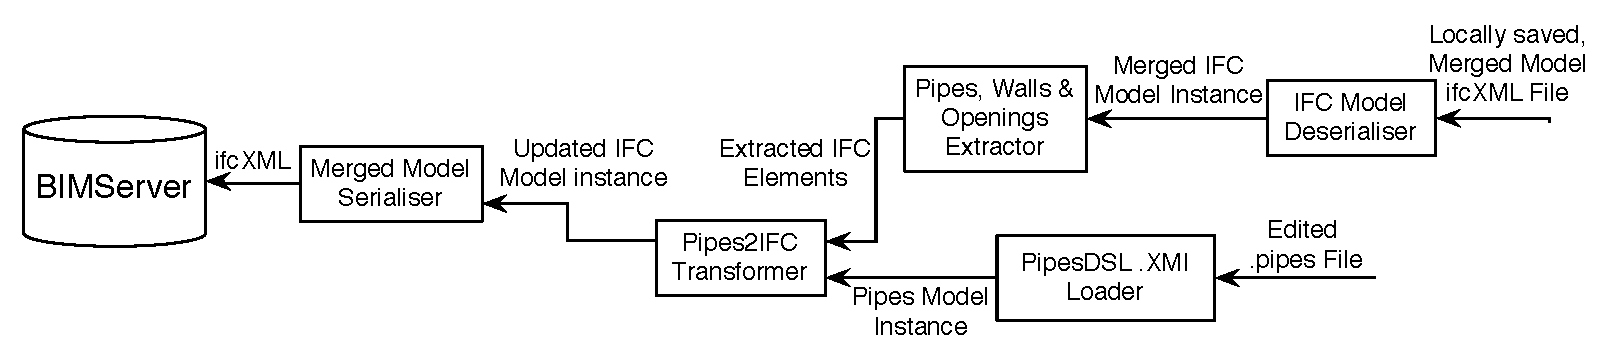
\includegraphics[width=120mm]{images/Pipes2IFC.pdf}
    \caption{Client-side workflow. First it updates the main IFC model with the changes written in the Pipes DSL editor, then sends the main model back to BIMServer.}
    \label{fig:Pipes2IFCWorkflow}
\end{figure}

Clearly, most of the work in this workflow lies with the Main Model Updater, which uses a pattern match-like dispatch language feature of Xtend to elegantly update the Java object graph of the extracted model. The routine runs through all elements in the Java object graph to update the corresponding Pipes DSL objects by looking at matching GUIDs. Only traversing an extract of the main model guarantees a better running time and still guarantees a correct update procedure, as the Pipes DSL does not allow any updates to elements outside of this extract anyway.

\subsubsection{Adding and Removing} The setup not only supports updating the attributes of elements, it also allows the user to do structural changes on the model. The Main Model Updater looks for elements in the Pipes DSL object graph without a GUID to determine if a new element should be created in the IFC model. This feature allows the user to add missing openings for pipe segments and is therefore crucial for the usefulness of the end product.

Likewise, if the updater fails to find an element in Pipes DSL object graph that corresponds to the existing one in the Java object graph it means the element has been deleted and that the Main Model Updater should take appropriate action to update references
